\documentclass[twocolumn]{revtex4-2}
\usepackage{graphicx}
\usepackage{amsmath}
\usepackage{hyperref}
\usepackage{xcolor}

\newcommand{\Lagr}{\mathcal{L}}

\begin{document}

\date{\today}
\author{Sixten Nordegren}
\title{Chaos in the double pendulum}

\maketitle

\section{Introduction}
The purpose of this assignment is to find solutions to and solve the double pendulum system. And, beyond that analyze the chaotic behaviour that emerges from it. 
\begin{figure}[b]
	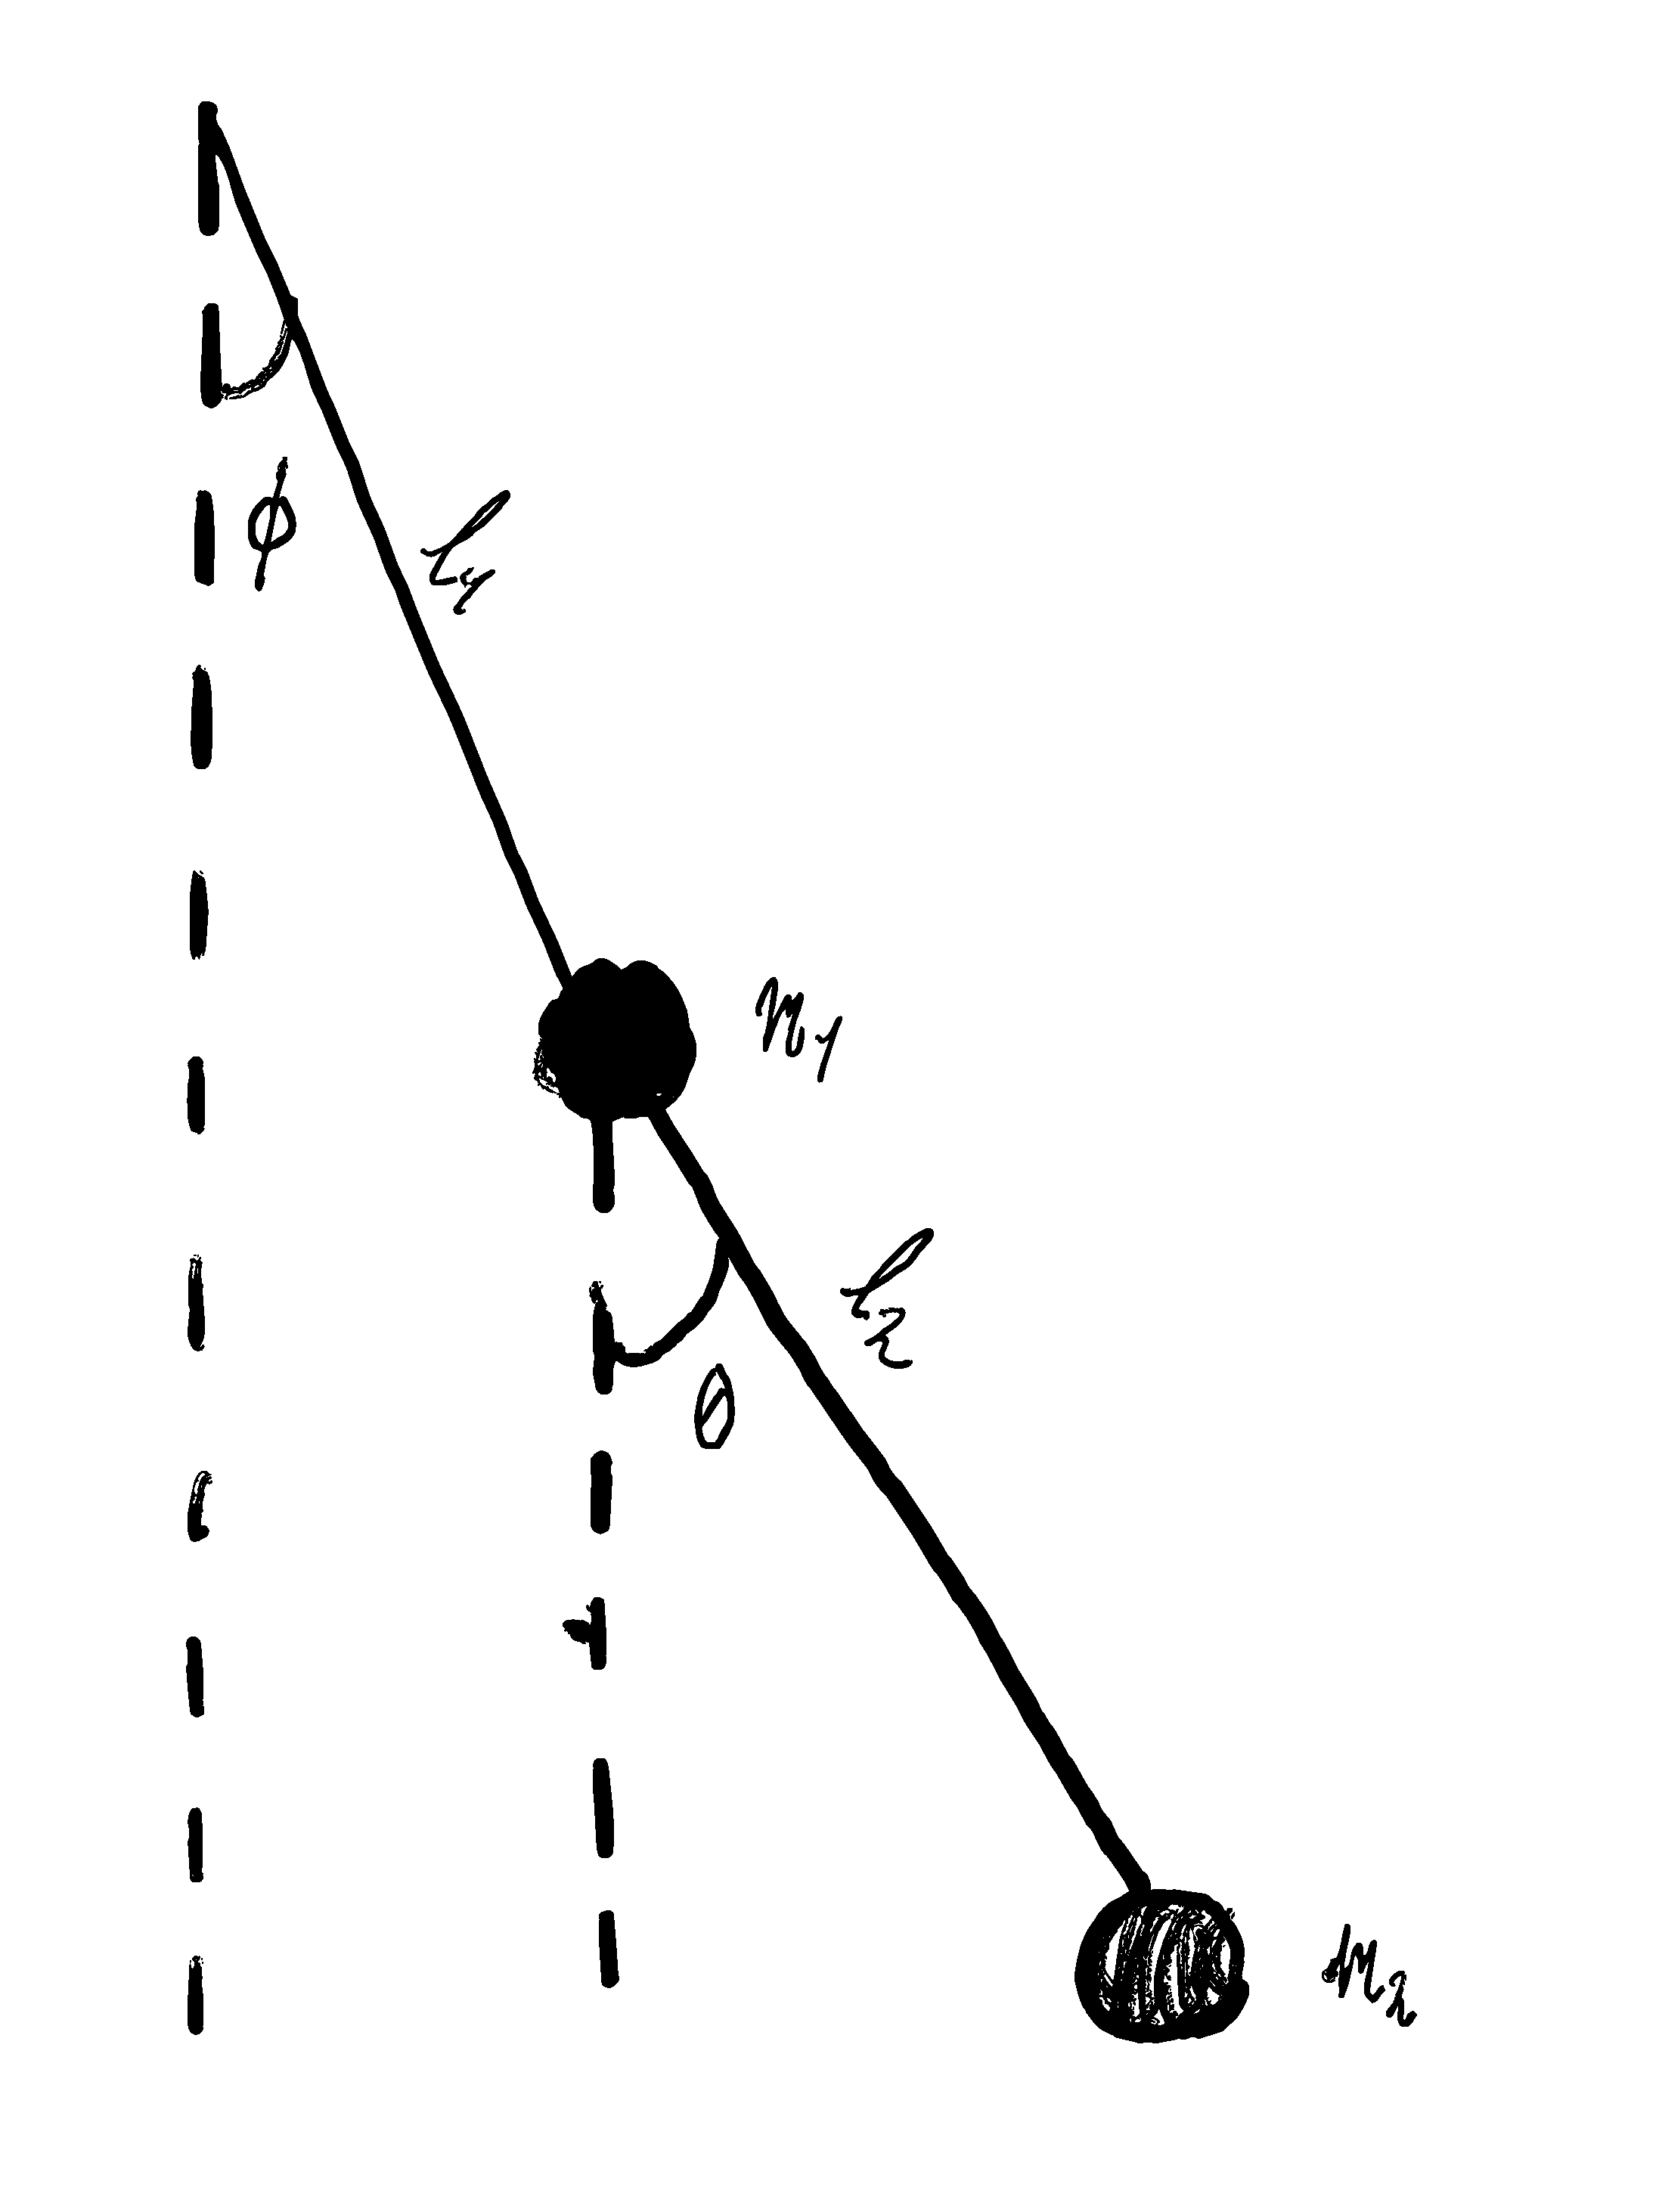
\includegraphics[width=0.5\linewidth]{~/Documents/anme/handin/test.pdf}
	\caption{Double pendulum \label{fig: doubble pendulum}}
\end{figure}
\section{Method}
\subsection{Lagrangian approach to the double pendulum}
Using the coordinates shown in \ref{fig: doubble pendulum}. We can observe that we have four degrees of freedom with two constraints. This leaves us with $4 - 2  = 2$ generalized coordinates required to describe the system. \footnote{Here we note that since the only conserved quantity is energy, we do in fact have one more degrees of freedom than conserved quantities. Indicative of a chaotic system.}

In the assignment, I took the liberty of assuming that the only objects in the systems that carry any mass is $m_1$ and $m_2$ marked in \ref{fig: doubble pendulum}. This means that the only part of the system that can hold any energy is those masses. I now then proceed to write out the position vectors of those masses.
\begin{align*}
	r_1 &= (l_1 \sin{(\phi)}, l_1 \cos{(\phi)}) \\
	r_2 &= (l_1 \sin{(\phi)} + l_2 \sin{(\theta)}, l_1 \cos{(\phi)} + l_2\cos{(\theta)})
\end{align*}
Now that we have the position vectors we are ready to try and write the Lagrangian $(\Lagr)$.

\begin{equation}
	\Lagr = \frac{1}{2}m\dot r_1^2 + \frac{1}{2}m\dot r_2^2 - V_1 - V_2
	\label{eq: Lagrangian initial}
\end{equation}
\begin{align}
	V_1 &= m_1gl_1(1 - \cos{(\phi)}) \nonumber \\
	V_2 &= m_2g(l_1(1 - \cos{(\phi)}) + l_2(1 - \cos{(\theta)}) )
	\label{eq: init pot}
\end{align}
This expression carries terms that are just constants (If you would to multiply in the factors outside of the parentheses) which later on, in the Euler-Lagrange equations cancel. For this reason, any further reference to \ref{eq: init pot} will be made without them. \footnote{From what I can tell, this is the standard way of treating the constants to parts of the Lagrangian that ends up disappearing. Typically, without any reference to doing so whatsoever. Which I personally find very confusing. So I decided to include a small paragraph notifying the reader of doing so.}
\begin{align*}
	\dot r_1^2 &= ( l_1 \dot \phi )^2 \\
	\dot r_2^2 &= l_1^2 \dot \phi ^2 + l_2 \dot \theta ^2 +... \\
		   &  ... + 2l_1l_2(
	\cos{(\phi)}\cos{(\theta)} + \sin{(\phi)}\sin{(\theta)}
	)\dot \phi \dot \theta
\end{align*}
Which turns \ref{eq: Lagrangian initial} into;

\begin{widetext}
	\begin{equation}
		\Lagr = \frac{m_1}{2}l_1 ^2 \dot \phi ^2 + \frac{ m_2 }{2}\left(l_1^2 \dot \phi ^2
		+ l_2^2 \dot \phi ^2 + 2l_1l_2(
	\cos{(\phi)}\cos{(\theta)} + \sin{(\phi)}\sin{(\theta)}
	)\dot \phi \dot \theta
\right) + g(m_1 + m_2)(\cos{(\phi)})l_1 + gm_2l_2(\cos{(\theta)})
	\end{equation}
\end{widetext}
We can shorten this expression slightly by using the identity $ \cos{(s)}\cos{(t)} + \sin{(s)}\sin{(t)}
= \cos{(s - t)}$ But it doesn't get more compact than that.

Now turning to the Euler-Lagrange equations: 
\begin{equation}
	\frac{\partial \Lagr}{\partial q_i} = \frac{d}{dt}\frac{\partial \Lagr}{\partial \dot q_i}
	\label{eq: E-L}
\end{equation}

\begin{align*}
	\frac{\partial \Lagr}{\partial \phi} &= - m_2l_1l_2\dot \phi \dot \theta \sin{(\phi - \theta)} -
	g(m_2+m_1)l_1\sin{(\phi)} \\
	\frac{\partial \Lagr}{\partial \theta} &=  m_2l_1l_2\dot \phi \dot \theta \sin{(\phi - \theta)} -
	gm_2l_1\sin{(\theta)} \\
	\frac{d}{dt}\left(\frac{\partial \Lagr}{\partial \dot \phi} \right) &= l_1^2(m_1 +m_2)\ddot \phi +
	m_2l_1l_2\ddot \theta\cos{(\phi - \theta)}
	 \\
	& \quad ... - m_2l_1l_2\dot \theta \sin{(\phi - \theta)}\dot \phi  + m_2l_1l_2
\dot \theta \dot \phi \sin{(\phi - \theta)} \\
	\frac{d}{dt} \left( \frac{\partial \Lagr}{\partial \dot \theta} \right) &= l_2^2m_2\ddot \theta +
	m_2l_1l_2\ddot \phi\cos{(\phi - \theta)}
	 \\
	& \quad ... - m_2l_1l_2\dot \phi^{2} \sin{(\phi - \theta)}  - m_2l_1l_2
\dot \theta \dot \phi \sin{(\phi - \theta)} \\
\end{align*}

\begin{widetext}
With these expressions we can now write \ref{eq: E-L} as:
	\begin{equation}
 -g(m_2+m_1)l_1\sin{(\phi)} = 
 l_1^2(m_1 +m_2)\ddot \phi +
	m_2l_1l_2\ddot \theta\cos{(\phi - \theta)} + m_2l_1l_2
\dot \theta \dot \phi \sin{(\phi - \theta)} 
	\label{eq: diff 1it 1}
	\end{equation}
	\begin{equation}
- gm_2l_1\sin{(\theta)}  = 
 l_2^2m_2\ddot \theta +
	m_2l_1l_2\ddot \phi\cos{(\phi - \theta)}
	- m_2l_1l_2\dot \phi^{2} \sin{(\phi - \theta)} 
	\label{eq: diff 1it 2}
	\end{equation}
\end{widetext}
These are nothing but a second degree differential equations. We could try to solve that but instead, the easier approach is to try and turn it into a first degree differential equation. We can do this by first using equations \ref{eq: diff 1it 1} and \ref{eq: diff 1it 2} as a linear systems of equations and solving for the second derivatives.\textcolor{red}{ I'll show this derivation in appendix \ref{ap: lin eq}.} Now defining new coordinates $\omega_1 = \dot \phi$ and $\omega_2 = \dot \theta$ allows us to write the following :
\begin{equation}
	\left(
	\begin{array}{c}
		\dot \phi \\
		\dot \theta \\
		\ddot \phi \\
		\ddot \theta
	\end{array} \right)  =
	\left(\begin{array}{c}
		\omega_1 \\
		\omega_2 \\
		g_1(\phi, \theta, \omega_1, \omega_2) \\
		g_2(\phi, \theta, \omega_1, \omega_2)
	\end{array}\right)
\end{equation}
\footnote{Definitions of $g_1$ and $g_2$ will be included in the appendix}.

This is precisely the form we need the differential equation to apply Runge-Kutta 4 on, for details see \cite{newman_2013}.\footnote{Anyone interested in how this was done specifically or seeing any of the code I wrote. You can find all of it on \url{https://github.com/SixtenNordegren/DoubblePendulum}.}

\begin{figure}[t]
	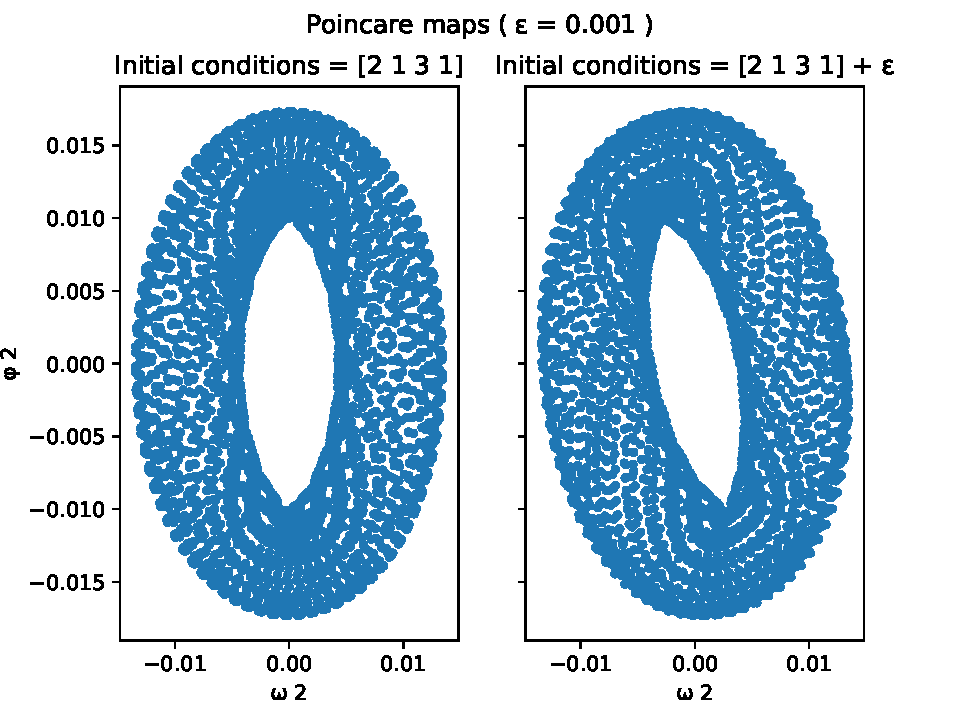
\includegraphics[width=\linewidth]{~/Documents/anme/handin/poincare_1.pdf}
	\caption{Poincare map \label{fig: poincare 1} with $3000$ points}
\end{figure}
\begin{figure}[b]
	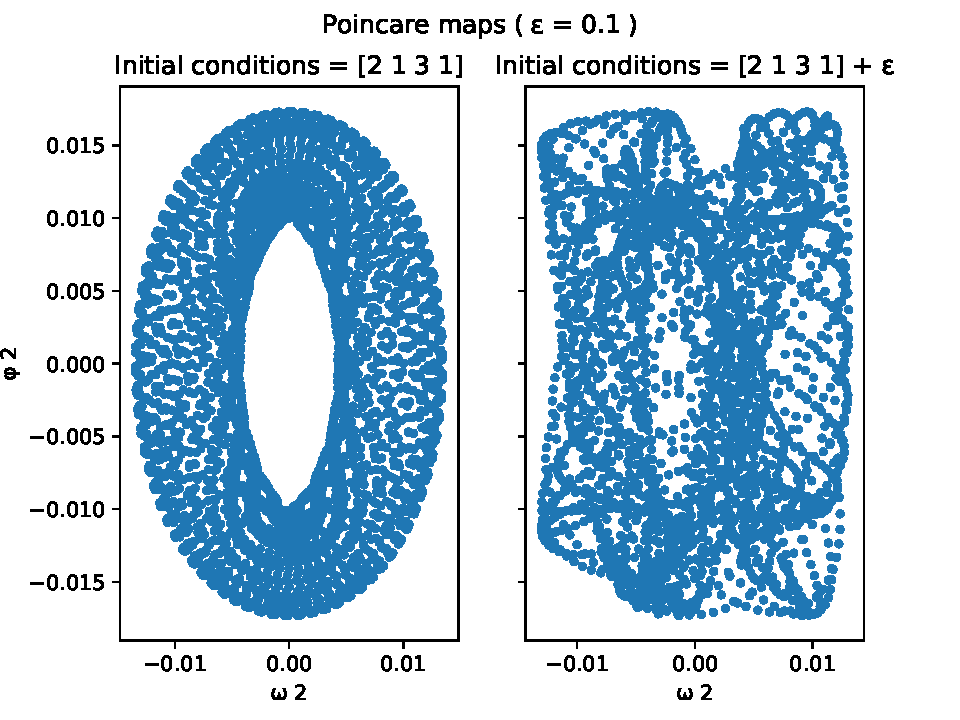
\includegraphics[width=\linewidth]{~/Documents/anme/handin/poincare_2.pdf}
	\caption{Poincare map \label{fig: poincare 2} with $3000$ points}
\end{figure}
There are two different types of initial conditions that we can manipulate. We can either change the masses and lengths of the rods. Alternatively, we could change the initial displacement of the generalized coordinates. This would correspond to lifting either of the bobs in the pendulum slightly before releasing it. It's the former of these two that we will manipulate to see how small changes affects the chaos of the system. Both would of course be of interest, but we shall have to contain our analysis somewhat for the sake of brevity.
\par
After solving the differential equation with the Runge-Kutta\cite{newman_2013} method we can plot our results in the form of Poincare maps. See \ref{fig: poincare 1}. Here we can see how drastic a difference a slight change in initial conditions ( a change of $\varepsilon$ in each of the parameters of the set of initial conditions ) can have on the outcome of the total system. To underline this point even more one can observe what happens when the initial disruption is changed from $\varepsilon = 0.001 $ to $\varepsilon = 0.1$. What previously caused a shift in the structure of the system, has now become a completely unrecognizable one.

\section{Summary}
It seems that the pendulum is indeed chaotic. Closer analysis of how it's chaotic remains to be done. For further analysis one could look at Lyapunov exponents to try and quantify the chaotic behaviour somewhat. One could also look at how changing the initial conditions of the generalized coordinates changes the system.
\newpage
\appendix 
\section{Solution of system of linear equation for Euler-Lagrange equations }
\label{ap: lin eq}
We can write equations \ref{eq: diff 1it 1} and \ref{eq: diff 1it 2} as:
\begin{align}
	\ddot \phi& + \ddot \theta \frac{m_2l_2\cos{(\phi -\theta)}}{(m_1 + m_2)l_1} = -\frac{g\sin{(\phi)}}{l_1} - \frac{m_2 l_2 \dot \theta^{2} }{(m_1 + m_2)l_1} \\
	\ddot \theta& + \ddot \phi \frac{l_1}{l_2}\cos{(\phi - \theta)} = \frac{l_1}{l_2}\dot \phi^2\sin{(\phi - \theta)} - \frac{g}{l_2}\sin{(\theta)}
\end{align}

Or equivalently: \footnote{The idea to write out the equations in different terms of the functions of 
the respective 2'nd derivatives was something I found on a blog, written by a guy named Diego Assencio. \url{https://diego.assencio.com/?index=1500c66ae7ab27bb0106467c68feebc6}}
\begin{align}
	\ddot \phi & + \ddot \theta \alpha_1 = f_1 \\
	\ddot \theta & + \ddot \alpha_2 = f_2
\end{align}
With, 
\begin{align}
	\alpha_1 &= \frac{m_2l_2\cos{(\phi -\theta)}}{(m_1 + m_2)l_1} \\
	f_1 &= -\frac{g\sin{(\phi)}}{l_1} - \frac{m_2 l_2 \dot \theta^{2} }{(m_1 + m_2)l_1} \\
	\alpha_2 &= \frac{l_1}{l_2}\cos{(\phi - \theta)} \\
	f_2 &= \frac{l_1}{l_2}\dot \phi^2\sin{(\phi - \theta)} - \frac{g}{l_2}\sin{(\theta)}
\end{align}

We can solve this like any other system of linear equations.

\begin{equation}
\left(\begin{array}{c c | c}
1 & \alpha_1 & f_1 \\
\alpha_2 & 1 & f_2
\end{array}\right) \sim
\left(\begin{array}{c c | c}
1 & 0 & \frac{-f_1+f_2\alpha_1}{\alpha_1\alpha_2-1} \\
0 & 1 & \frac{-f_2+f_1\alpha_2}{\alpha_1\alpha_2-1}
\end{array}\right)
\end{equation}
So we have 
\begin{align}
	g_1(\phi, \theta,\dot \phi,\dot \theta) = \frac{-f_1+f_2\alpha_1}{\alpha_1\alpha_2-1} \\
	g_2(\phi, \theta,\dot \phi,\dot \theta) = \frac{-f_2+f_1\alpha_2}{\alpha_1\alpha_2-1}
\end{align}
\bibliography{bibliography}
\end{document}

